\begin{figure}
	\centering
	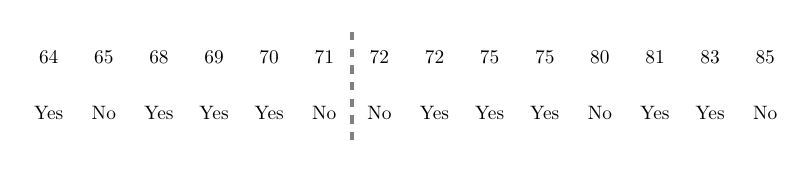
\begin{tikzpicture}[
		scale=0.7,
		every node/.style={scale=0.7}
	]

		\foreach \x/\v/\l in {
			1/64/Yes,2/65/No,3/68/Yes,4/69/Yes,5/70/Yes,6/71/No,7/72/No,
			8/72/Yes,9/75/Yes,10/75/Yes,11/80/No,12/81/Yes,13/83/Yes,14/85/No}{
			\node at (\x, 0) {\highlight{\v}};
			\node at (\x, -1) {\highlight{\l}};
		}

		\draw[gray,dashed,ultra thick] (6.5,-1.5) -- (6.5,0.5);
		
	\end{tikzpicture}
\end{figure}